% Options for packages loaded elsewhere
% Options for packages loaded elsewhere
\PassOptionsToPackage{unicode}{hyperref}
\PassOptionsToPackage{hyphens}{url}
\PassOptionsToPackage{dvipsnames,svgnames,x11names}{xcolor}
%
\documentclass[
  letterpaper,
  DIV=11,
  numbers=noendperiod]{scrartcl}
\usepackage{xcolor}
\usepackage{amsmath,amssymb}
\setcounter{secnumdepth}{-\maxdimen} % remove section numbering
\usepackage{iftex}
\ifPDFTeX
  \usepackage[T1]{fontenc}
  \usepackage[utf8]{inputenc}
  \usepackage{textcomp} % provide euro and other symbols
\else % if luatex or xetex
  \usepackage{unicode-math} % this also loads fontspec
  \defaultfontfeatures{Scale=MatchLowercase}
  \defaultfontfeatures[\rmfamily]{Ligatures=TeX,Scale=1}
\fi
\usepackage{lmodern}
\ifPDFTeX\else
  % xetex/luatex font selection
\fi
% Use upquote if available, for straight quotes in verbatim environments
\IfFileExists{upquote.sty}{\usepackage{upquote}}{}
\IfFileExists{microtype.sty}{% use microtype if available
  \usepackage[]{microtype}
  \UseMicrotypeSet[protrusion]{basicmath} % disable protrusion for tt fonts
}{}
\makeatletter
\@ifundefined{KOMAClassName}{% if non-KOMA class
  \IfFileExists{parskip.sty}{%
    \usepackage{parskip}
  }{% else
    \setlength{\parindent}{0pt}
    \setlength{\parskip}{6pt plus 2pt minus 1pt}}
}{% if KOMA class
  \KOMAoptions{parskip=half}}
\makeatother
% Make \paragraph and \subparagraph free-standing
\makeatletter
\ifx\paragraph\undefined\else
  \let\oldparagraph\paragraph
  \renewcommand{\paragraph}{
    \@ifstar
      \xxxParagraphStar
      \xxxParagraphNoStar
  }
  \newcommand{\xxxParagraphStar}[1]{\oldparagraph*{#1}\mbox{}}
  \newcommand{\xxxParagraphNoStar}[1]{\oldparagraph{#1}\mbox{}}
\fi
\ifx\subparagraph\undefined\else
  \let\oldsubparagraph\subparagraph
  \renewcommand{\subparagraph}{
    \@ifstar
      \xxxSubParagraphStar
      \xxxSubParagraphNoStar
  }
  \newcommand{\xxxSubParagraphStar}[1]{\oldsubparagraph*{#1}\mbox{}}
  \newcommand{\xxxSubParagraphNoStar}[1]{\oldsubparagraph{#1}\mbox{}}
\fi
\makeatother

\usepackage{color}
\usepackage{fancyvrb}
\newcommand{\VerbBar}{|}
\newcommand{\VERB}{\Verb[commandchars=\\\{\}]}
\DefineVerbatimEnvironment{Highlighting}{Verbatim}{commandchars=\\\{\}}
% Add ',fontsize=\small' for more characters per line
\usepackage{framed}
\definecolor{shadecolor}{RGB}{241,243,245}
\newenvironment{Shaded}{\begin{snugshade}}{\end{snugshade}}
\newcommand{\AlertTok}[1]{\textcolor[rgb]{0.68,0.00,0.00}{#1}}
\newcommand{\AnnotationTok}[1]{\textcolor[rgb]{0.37,0.37,0.37}{#1}}
\newcommand{\AttributeTok}[1]{\textcolor[rgb]{0.40,0.45,0.13}{#1}}
\newcommand{\BaseNTok}[1]{\textcolor[rgb]{0.68,0.00,0.00}{#1}}
\newcommand{\BuiltInTok}[1]{\textcolor[rgb]{0.00,0.23,0.31}{#1}}
\newcommand{\CharTok}[1]{\textcolor[rgb]{0.13,0.47,0.30}{#1}}
\newcommand{\CommentTok}[1]{\textcolor[rgb]{0.37,0.37,0.37}{#1}}
\newcommand{\CommentVarTok}[1]{\textcolor[rgb]{0.37,0.37,0.37}{\textit{#1}}}
\newcommand{\ConstantTok}[1]{\textcolor[rgb]{0.56,0.35,0.01}{#1}}
\newcommand{\ControlFlowTok}[1]{\textcolor[rgb]{0.00,0.23,0.31}{\textbf{#1}}}
\newcommand{\DataTypeTok}[1]{\textcolor[rgb]{0.68,0.00,0.00}{#1}}
\newcommand{\DecValTok}[1]{\textcolor[rgb]{0.68,0.00,0.00}{#1}}
\newcommand{\DocumentationTok}[1]{\textcolor[rgb]{0.37,0.37,0.37}{\textit{#1}}}
\newcommand{\ErrorTok}[1]{\textcolor[rgb]{0.68,0.00,0.00}{#1}}
\newcommand{\ExtensionTok}[1]{\textcolor[rgb]{0.00,0.23,0.31}{#1}}
\newcommand{\FloatTok}[1]{\textcolor[rgb]{0.68,0.00,0.00}{#1}}
\newcommand{\FunctionTok}[1]{\textcolor[rgb]{0.28,0.35,0.67}{#1}}
\newcommand{\ImportTok}[1]{\textcolor[rgb]{0.00,0.46,0.62}{#1}}
\newcommand{\InformationTok}[1]{\textcolor[rgb]{0.37,0.37,0.37}{#1}}
\newcommand{\KeywordTok}[1]{\textcolor[rgb]{0.00,0.23,0.31}{\textbf{#1}}}
\newcommand{\NormalTok}[1]{\textcolor[rgb]{0.00,0.23,0.31}{#1}}
\newcommand{\OperatorTok}[1]{\textcolor[rgb]{0.37,0.37,0.37}{#1}}
\newcommand{\OtherTok}[1]{\textcolor[rgb]{0.00,0.23,0.31}{#1}}
\newcommand{\PreprocessorTok}[1]{\textcolor[rgb]{0.68,0.00,0.00}{#1}}
\newcommand{\RegionMarkerTok}[1]{\textcolor[rgb]{0.00,0.23,0.31}{#1}}
\newcommand{\SpecialCharTok}[1]{\textcolor[rgb]{0.37,0.37,0.37}{#1}}
\newcommand{\SpecialStringTok}[1]{\textcolor[rgb]{0.13,0.47,0.30}{#1}}
\newcommand{\StringTok}[1]{\textcolor[rgb]{0.13,0.47,0.30}{#1}}
\newcommand{\VariableTok}[1]{\textcolor[rgb]{0.07,0.07,0.07}{#1}}
\newcommand{\VerbatimStringTok}[1]{\textcolor[rgb]{0.13,0.47,0.30}{#1}}
\newcommand{\WarningTok}[1]{\textcolor[rgb]{0.37,0.37,0.37}{\textit{#1}}}

\usepackage{longtable,booktabs,array}
\newcounter{none} % for unnumbered tables
\usepackage{calc} % for calculating minipage widths
% Correct order of tables after \paragraph or \subparagraph
\usepackage{etoolbox}
\makeatletter
\patchcmd\longtable{\par}{\if@noskipsec\mbox{}\fi\par}{}{}
\makeatother
% Allow footnotes in longtable head/foot
\IfFileExists{footnotehyper.sty}{\usepackage{footnotehyper}}{\usepackage{footnote}}
\makesavenoteenv{longtable}
\usepackage{graphicx}
\makeatletter
\newsavebox\pandoc@box
\newcommand*\pandocbounded[1]{% scales image to fit in text height/width
  \sbox\pandoc@box{#1}%
  \Gscale@div\@tempa{\textheight}{\dimexpr\ht\pandoc@box+\dp\pandoc@box\relax}%
  \Gscale@div\@tempb{\linewidth}{\wd\pandoc@box}%
  \ifdim\@tempb\p@<\@tempa\p@\let\@tempa\@tempb\fi% select the smaller of both
  \ifdim\@tempa\p@<\p@\scalebox{\@tempa}{\usebox\pandoc@box}%
  \else\usebox{\pandoc@box}%
  \fi%
}
% Set default figure placement to htbp
\def\fps@figure{htbp}
\makeatother





\setlength{\emergencystretch}{3em} % prevent overfull lines

\providecommand{\tightlist}{%
  \setlength{\itemsep}{0pt}\setlength{\parskip}{0pt}}



 


\usepackage{booktabs}
\usepackage{longtable}
\usepackage{array}
\usepackage{multirow}
\usepackage{wrapfig}
\usepackage{float}
\usepackage{colortbl}
\usepackage{pdflscape}
\usepackage{tabu}
\usepackage{threeparttable}
\usepackage{threeparttablex}
\usepackage[normalem]{ulem}
\usepackage{makecell}
\usepackage{xcolor}
\KOMAoption{captions}{tableheading}
\makeatletter
\@ifpackageloaded{caption}{}{\usepackage{caption}}
\AtBeginDocument{%
\ifdefined\contentsname
  \renewcommand*\contentsname{Table of contents}
\else
  \newcommand\contentsname{Table of contents}
\fi
\ifdefined\listfigurename
  \renewcommand*\listfigurename{List of Figures}
\else
  \newcommand\listfigurename{List of Figures}
\fi
\ifdefined\listtablename
  \renewcommand*\listtablename{List of Tables}
\else
  \newcommand\listtablename{List of Tables}
\fi
\ifdefined\figurename
  \renewcommand*\figurename{Figure}
\else
  \newcommand\figurename{Figure}
\fi
\ifdefined\tablename
  \renewcommand*\tablename{Table}
\else
  \newcommand\tablename{Table}
\fi
}
\@ifpackageloaded{float}{}{\usepackage{float}}
\floatstyle{ruled}
\@ifundefined{c@chapter}{\newfloat{codelisting}{h}{lop}}{\newfloat{codelisting}{h}{lop}[chapter]}
\floatname{codelisting}{Listing}
\newcommand*\listoflistings{\listof{codelisting}{List of Listings}}
\makeatother
\makeatletter
\makeatother
\makeatletter
\@ifpackageloaded{caption}{}{\usepackage{caption}}
\@ifpackageloaded{subcaption}{}{\usepackage{subcaption}}
\makeatother
\usepackage{bookmark}
\IfFileExists{xurl.sty}{\usepackage{xurl}}{} % add URL line breaks if available
\urlstyle{same}
\hypersetup{
  pdftitle={Glider Deployment Report: unit\_1024 (March 9th{,} 2026)},
  colorlinks=true,
  linkcolor={blue},
  filecolor={Maroon},
  citecolor={Blue},
  urlcolor={Blue},
  pdfcreator={LaTeX via pandoc}}


\title{Glider Deployment Report: unit\_1024 (March 9th, 2026)}
\author{}
\date{}
\begin{document}
\maketitle

\renewcommand*\contentsname{Table of contents}
{
\setcounter{tocdepth}{3}
\tableofcontents
}

\subsubsection{Summary}\label{summary}

The Ecosystem Science Division (ESD) at the Southwest Fisheries Science
Center (SWFSC) deployed glider \textbf{glider} (serial number) on
2026-03-09 off the coast of \textbf{location}
(33.17\textsuperscript{o}N, -117.49\textsuperscript{o}W) (Figure 1).
Sensors deployed on the glider are listed in Table~\ref{tbl-sensors}.

Figure~\ref{fig-map-1} (A) displays tracklines of glider during
deployment, while (B) displays the broad deployment area. The glider
remained deployed for 2 days, performed 24 dives, and traveled a total
of 10.91 km while diving to a maximum depth of 203 m. The glider was
recovered on 2026-03-10.

\begin{figure}

\centering{

\pandocbounded{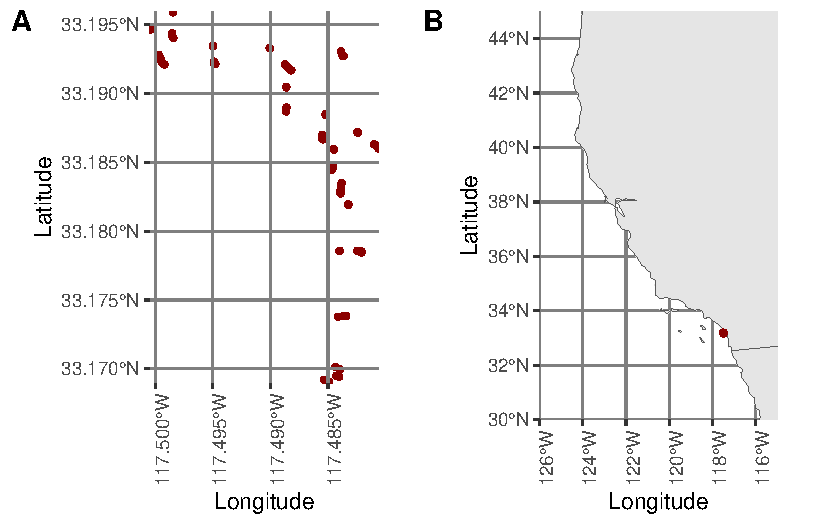
\includegraphics[keepaspectratio,alt={The map on the left shows a close-up display of where the glider surfaced throughout its deployment. The map on the right is zoomed out to show the approximate location of the glider deployment relative to land.}]{unit_1024-20260309_files/figure-pdf/fig-map-1-1.pdf}}

}

\caption{\label{fig-map-1}Glider tracklines. A displays close-up
tracklines, while B displays the broad deployment area.}

\end{figure}%

\begin{table}

\caption{\label{tbl-sensors}Science sampling strategies for current
glider deployment. Additional settings for the AZFP echosounder, the
Williamson and Associates camera, and the Nortek echosounder (if
installed) are defined in configuration and initialization files on the
glider's science computer, and are also housed on the Google Cloud
Platform. All deployment files are available on request.}

\centering{

\begin{tabular}{>{\raggedright\arraybackslash}p{1in}>{\raggedright\arraybackslash}p{2in}>{\raggedright\arraybackslash}p{1in}>{\raggedright\arraybackslash}p{1in}>{\raggedright\arraybackslash}p{1in}}
\toprule
File Name & Sensor & State to Sample & Depth to Sample & Serial Number\\
\midrule
\cellcolor{gray!15}{sample01.ma} & \cellcolor{gray!15}{Sea-Bird Conductivity Temperature Depth (CTD) (SBE-41)} & \cellcolor{gray!15}{See Table 2} & \cellcolor{gray!15}{1000 m} & \cellcolor{gray!15}{9715}\\
sample48.ma & Sea-Bird ECO Puck (backscatter and fluorescence) (FLBBCD-SLC, CDOM) & See Table 2 & 1000 m & 6866\\
\cellcolor{gray!15}{sample54.ma} & \cellcolor{gray!15}{AANDERAA oxygen optode (4831)} & \cellcolor{gray!15}{See Table 2} & \cellcolor{gray!15}{1000 m} & \cellcolor{gray!15}{1160}\\
sample87.ma & Shadowgraph camera (Williamson and Associates) & Diving, hovering, climbing & 1000 m & SG-V3-003\\
\bottomrule
\end{tabular}

}

\end{table}%

The glider was deployed in tandem with a second glider (``stenella'').
Each glider was equipped with a different passive acoustic monitor
(PAM), and the goals of this deployment were to 1) compare passive
acoustic data between the two sensors; 2) evaluate any potential
interference in passive acoustic data caused by other sensors on the
gliders, and 3) determine battery consumption of new sensors (passive
acoustic and photosynthetically active radiation sensors). All sensors
except PAMs were systematically turned off and on throughout the
deployment to isolate interference and to better assess battery usage.

\subsubsection{Introduction}\label{introduction}

The Ecosystem Science Division at NOAA Fisheries' Southwest Fisheries
Science Center monitors the living marine resources within the Southern
Ocean and the California Current in order to satisfy the requirements of
several legislative mandates to support conservation and management
decision-making. To achieve this goal, we use autonomous underwater
buoyancy-driven gliders with integrated sensors for measuring ocean
conditions, plankton densities, and marine mammal distributions.

Depending on the specific deployment objective, Slocum gliders are
equipped with a suite of sensors. We obtain acoustic estimates of
zooplankton density (primarily Antarctic krill in the Southern Ocean)
using one of two different echosounders: an Acoustic Zooplankton Fish
Profiler with discrete frequencies at 67.5 and 125 kHz (AZFP, ASL, Inc)
and a mini-Signature 100 wideband echosounder with continuous
frequencies between 70 and 120 kHz (Nortek). We also collect ancillary
oceanographic data (temperature, salinity, dissolved oxygen,
chlorophyll, colored dissolved organic matter, backscatter, and
photosynthetically active radiation) to characterize the marine
environment. Additional sensors may include passive acoustic monitors
for marine mammal detection (``Wispr'', Embedded Ocean Systems; digital
acoustic monitoring ``DMON'', Woods Hole Oceanographic Institution),
``glidercams'' for verifying acoustic targets (Williamson and
Associates, Inc.) and shadowgraph cameras for obtaining imagery of the
plankton community (Williamson and Associates, Inc.). Imagery is used to
train artificial intelligence (AI) models to automate plankton
identification.

Hefring OceanScout gliders are equipped with
conductivity-temperature-depth sensors (CTDs; RBR, Inc.) and ``Wispr''
passive acoustic monitors.

\subsubsection{Pre-Deployment Preparation and
Testing}\label{pre-deployment-preparation-and-testing}

Prior to deployment, the ESD has a standard protocol for preparing and
testing gliders to minimize or eliminate issues that may occur due to
human error during deployment:

\emph{Slocum gliders}

\begin{enumerate}
\def\labelenumi{\arabic{enumi}.}
\tightlist
\item
  Gliders are properly ballasted (i.e., weighted) so that the density of
  the glider matches the density of the water in which it will be
  deployed. Weight and flotation configurations are documented
\item
  The junctions between glider sections are thoroughly cleaned, old
  o-rings are discarded, new o-rings are inspected for damage that may
  compromise their ability to form a water-tight seal, new o-rings are
  properly lubricated, and the glider is sealed together. All cable
  connections are photographed to document the ``final seal'' and ensure
  the glider was reassembled properly
\item
  A ``Functional Checkout'' is performed to ensure and document that all
  glider systems and science sensors are functioning properly. During
  the Functional Checkout, we verify the battery type installed in the
  glider (lithium primary or lithium rechargeable) and that the
  appropriate battery duration (total coulomb amp hours) is active in
  the glider's autoexec.mi file
\item
  Two test missions are performed in the SWFSC test tank (20 m x 10 m x
  10 m) to ensure the glider is performing as expected
\item
  Once per year, glider compasses are calibrated (the compass was not
  calibrated prior to this deployment)
\item
  Biofouling prevention measures are applied as necessary
\item
  Glider flight and science sampling files are prepared according to
  mission objectives. These objectives are identified by the Principal
  Investigators for each deployment. Files are uploaded to the Teledyne
  Webb Research Slocum Fleet Mission Control (SFMC) web interface and
  sent to the glider just prior to deployment over the Iridium
  connection
\item
  When gliders are shipped to their deployment location, ESD glider
  technicians perform a second Functional Checkout to ensure the gliders
  function properly after transit
\end{enumerate}

\emph{OceanScout gliders}

\begin{enumerate}
\def\labelenumi{\arabic{enumi}.}
\tightlist
\item
  Gliders are configured with the standard ballast for salt water (8
  weights in the nose)
\item
  O-rings are replaced as needed
\item
  Motors (variable buoyancy engine, pitch, and roll) are calibrated,
  either through the glider's wifi connection prior to deployment, or by
  using platform.test through the command line interface
\item
  Routes, diving parameters, and sensor sampling strategies are
  established through the Hefring cloud interface and deployed to the
  glider
\end{enumerate}

\subsubsection{Deployment-specific
testing}\label{deployment-specific-testing}

ESD staff prepared this glider for deployment in February 2025; however,
during the Functional Checkout procedure, the valve in the oil pump did
not appear to be opening and closing properly (set\_for\_ballasting():
Error valve never closed). Teledyne staff were on site and ran repeated
tests, including a recalibration of the oil pump. Teledyne advised
against a deployment, as this valve issue may have prevented the glider
from pumping oil into the nose to inflect at depth, resulting in the
glider sinking and dispatching its ejection weight. The forward section
was returned to Teledyne for service. ESD staff swapped out the faulty
forward section (SN 0688) for a different forward section (SN 0693).
During the Functional Checkout procedure prior to the current
deployment, the valve issue was observed again and was reproducible only
after issuing the ``ballast'' command after an exit reset (when the oil
was retracting to its neutral position). Staff performed an extended
``wiggle'' and watched the oil volume change on the computer terminal
and did not observe the valve issue again. ESD staff determined that it
was safe to proceed with deployment (see March 3, 2025 email ``NOAA Unit
1025 Valve Issue'').

\subsubsection{Deployment}\label{deployment}

``glider'' was deployed on 2026-03-09, approximately 5 km west of
Mission Bay in the Pacific Ocean (33.17\textsuperscript{o}N,
-117.49\textsuperscript{o}W) from the ESD Zodiac R/V \emph{Ernest II}.
This glider was deployed with the sensor configuration listed above, and
with lithium rechargeable batteries (coulomb amp hour total = 215, no
extended energy bay). We began this deployment using the autoballast
feature to maximize oil pump efficiency. Autoballast converged
successfully early on and remained converged for the duration of the
deployment.

Because Randome digifins are sensitive to slight movements and produce
erroneous oddities that can lead to mission aborts, the following
commands were issued to the glider prior to sequencing our standard
mission (1k\_n.mi):

put u\_digifin\_hide\_oddities\_at\_surface 1

put u\_digifin\_mask\_movement\_warning\_at\_surface 1

The glider did not complete its first deployment test mission
(status.mi) successfully because m\_raw\_altitude was not reporting.
Pilots issued the ``use'' command and determined that the wrong
altimeter was installed in the glider's autoexec.mi file. Pilots fixed
the error and re-sent the autoexec.mi file to the glider, after which
status.mi completed normally. No other issues or problems were noted
during deployment activities.

One abort occurred during the deployment for a leak in the digifin,
approximately 5.5 hours after the glider was deployed. This issue has
been observed before, nearly always when the glider surfaces normally
for ``nothing commanded'' and is reading a surfacing script. While
digifins are unlikely to leak, pilots exercised caution and obtained
several digifin leakdetect readings to ensure all values were within
normal range (greater than 1019). The low value that triggered the abort
did not appear on the surface sensor plot or in the .sbd file, further
confirming that the leak was false. Pilots commanded the fin to 0.3 and
-0.3 and the measured values matched. Pilots then resequenced the
mission and started with one dive to 50 m to ensure the fin was
functioning properly. When the glider surfaced after the 50 m dive,
pilots paused the surfacing script and issued the following command:

!put u\_digifin\_leakdetect\_count 10

This command increases the number of consecutive leakdetect readings the
glider requires to abort its mission from the masterdata default of 5 to
10. While low digifin leakdetect readings were observed in the surface
dialogue on subsequent surfacings, they always rebounded to normal
values almost immediately and did not cause any additional aborts. We
did not observe any evidence of a leak in the fin upon recovery.

This glider performed well for the entire 15-day mission. The glider
used 7.55 amp hours over 15 days, or 2.52\% of its battery capacity.

Throughout the deployment, pilots systematically turned all science
sensors (except the PAM) on and off to evaluate whether noise from these
sensors affected the quality of PAM data. The PAM remained on for the
duration of the deployment. Other sensors were cycled on and off
according to Table 2. When sensors were on, they sampled only on dives.

\begin{longtable}[l]{llll}

\caption{\label{tbl-sampling}Sampling strategies for sensors to
determine whether individual sensors interfere with passive acoustic
data. Sensors were systematically turned off and on throughout the
deployment to isolate interence. Time is in UTC.}

\tabularnewline

\toprule
\cellcolor{gray!15}{Date} & \cellcolor{gray!15}{Time} & \cellcolor{gray!15}{Sensor} & \cellcolor{gray!15}{On.Off}\\


\bottomrule

\end{longtable}

\begin{Shaded}
\begin{Highlighting}[]
\NormalTok{\# \#| label: tbl{-}wispr}
\NormalTok{\# \#| tbl{-}cap: "Sensor settings for the \textquotesingle{}wispr\textquotesingle{} passive acoustic monitor to determine optimal settings. Settings were changed approximately every 12 hours for the last three days of the deployment. Time is in UTC."}
\NormalTok{\# \#| echo: false}
\NormalTok{\# \#| message: false}

\NormalTok{\# \#read each line of the list as a separate character string}
\NormalTok{\# pa.cfg\textless{}{-}lapply(here(base.path,deployment,"archive{-}sfmc",listpacfg),read\_lines)}

\NormalTok{\# \#unlist the list so that individual strings can be selected}
\NormalTok{\# pa.cfg\textless{}{-}unlist(pa.cfg)}

\NormalTok{\# \#select strings that start with "b\_arg:" (ma files),"$" (cfg files), a capital letter (ini files), or that don\textquotesingle{}t start with "\#" (proglets)}
\NormalTok{\# pa.cfg.args\textless{}{-}pa.cfg[grep("\^{}\textbackslash{}\textbackslash{}$ADC,.*",pa.cfg)] }

\NormalTok{\# \#create a dataframe so that a column with date/time stamp can be added}
\NormalTok{\# pa.cfg.args\textless{}{-}as.data.frame(pa.cfg.args)}

\NormalTok{\# \#split the original file names to isolate the date/time string}
\NormalTok{\# x2\textless{}{-}str\_split(listpacfg,"\_")}

\NormalTok{\# \#unlist the list so that individual strings can be selected}
\NormalTok{\# x2\textless{}{-}unlist(x2)}

\NormalTok{\# \#just select the date/time strings}
\NormalTok{\# x2\textless{}{-}x2[c(TRUE,FALSE)]}

\NormalTok{\# \#create new columns with date and time for each data frame}
\NormalTok{\# pa.cfg.args\textless{}{-}cbind(pa.cfg.args,x2)}

\NormalTok{\# \#create new data frame with all args}
\NormalTok{\# new.col.names\textless{}{-}c("value","date.time")}
\NormalTok{\# colnames(pa.cfg.args)\textless{}{-}new.col.names}

\NormalTok{\# \#splitting date and time}
\NormalTok{\# pa.cfg.args\textless{}{-}pa.cfg.args \%\textgreater{}\% separate\_wider\_delim(date.time,"T",names=c("Date","Time"))}
\NormalTok{\# pa.cfg.args\textless{}{-}as.data.frame(pa.cfg.args)}

\NormalTok{\# \#reorder columns}
\NormalTok{\# pa.cfg.args\textless{}{-}pa.cfg.args[,c(2,3,1)]}
\NormalTok{\# colnames(pa.cfg.args)\textless{}{-}c("Date","Time","Setting")}

\NormalTok{\# \#format date}
\NormalTok{\# pa.cfg.args$Date\textless{}{-}strptime(pa.cfg.args$Date,format="\%Y\%m\%d",tz="UTC")}

\NormalTok{\# \#reformat time}
\NormalTok{\# pa.cfg.args$Time\textless{}{-}strptime(pa.cfg.args$Time,format="\%H\%M\%S")}
\NormalTok{\# pa.cfg.args$Time\textless{}{-}strftime(pa.cfg.args$Time,"\%H:\%M:\%S")}

\NormalTok{\# \#insert backslashes to prevent values from printing as formulas}
\NormalTok{\# pa.cfg.args$Setting\textless{}{-}paste0("\textbackslash{}\textbackslash{}",pa.cfg.args$Setting)}

\NormalTok{\# knitr::kable(pa.cfg.args,format="latex",booktabs=TRUE,longtable=TRUE,linesep="") \%\textgreater{}\%}
\NormalTok{\#   kableExtra::kable\_styling(position="left",latex\_options="striped",stripe\_color="gray!15")}
\end{Highlighting}
\end{Shaded}

Unlike the ``Wispr'' PAM on the glider ``stenella,'' pilots are unable
to modify DMON settings during a deployment. DMON settings were
configured prior to deployment for continuous recording of the
low-frequency hydrophone at 2 kHz and duty-cycled recording of the
high-frequency hydrophone at 120 kHz for 30 seconds out of every 450
seconds.

\subsubsection{Post-deployment actions}\label{post-deployment-actions}

Once the glider was back in the laboratory, pilots attempted downloading
data using the comms cable connection and the high-speed setting that
allows us to maximize the baud rate of the freewave (hs on). Pilots
found that they were unable to communicate with the glider over the ZOC
terminal once the comms cable was connected, even if the USB end of the
cable was not connected to the computer. Pilots tried switching comm
ports between the freewave and the comms cable on the computer without
success. Pilots tried using Tera Term instead of ZOC and were able to
communicate with the glider after the comms cable was connected and to
switch to the high baud rate, but the connection repeatedly timed out
when pilots attempted to download data and no files were transferred.
Pilots opened the glider and downloaded all data directly from SD cards.
Pilots suspect the issue may be related to the software version and will
investigate.

Calculations related to battery consumption remain to be done.

\subsubsection{Figures}\label{figures}

Plots below are generated from raw data which has not yet been
quality-checked.

\pandocbounded{\includegraphics[keepaspectratio,alt={a}]{\%60\%7Br\%7D bs\%60.pdf}}
\pandocbounded{\includegraphics[keepaspectratio,alt={b}]{\%60\%7Br\%7D chl\%60.pdf}}
\pandocbounded{\includegraphics[keepaspectratio,alt={c}]{\%60\%7Br\%7D den\%60.pdf}}
\pandocbounded{\includegraphics[keepaspectratio,alt={d}]{\%60\%7Br\%7D oxy\%60.pdf}}
\pandocbounded{\includegraphics[keepaspectratio,alt={e}]{\%60\%7Br\%7D sal\%60.pdf}}
\pandocbounded{\includegraphics[keepaspectratio,alt={f}]{\%60\%7Br\%7D temp\%60.pdf}}




\end{document}
